%\subsection{Исследование предметной области}
\begin{frame}[shrink=20]%[plain, noframenumbering, t, shrink=20]
\frametitle{Исследование предметной области}
    \vspace{-2ex} 
    \begin{figure}[!htbp]
        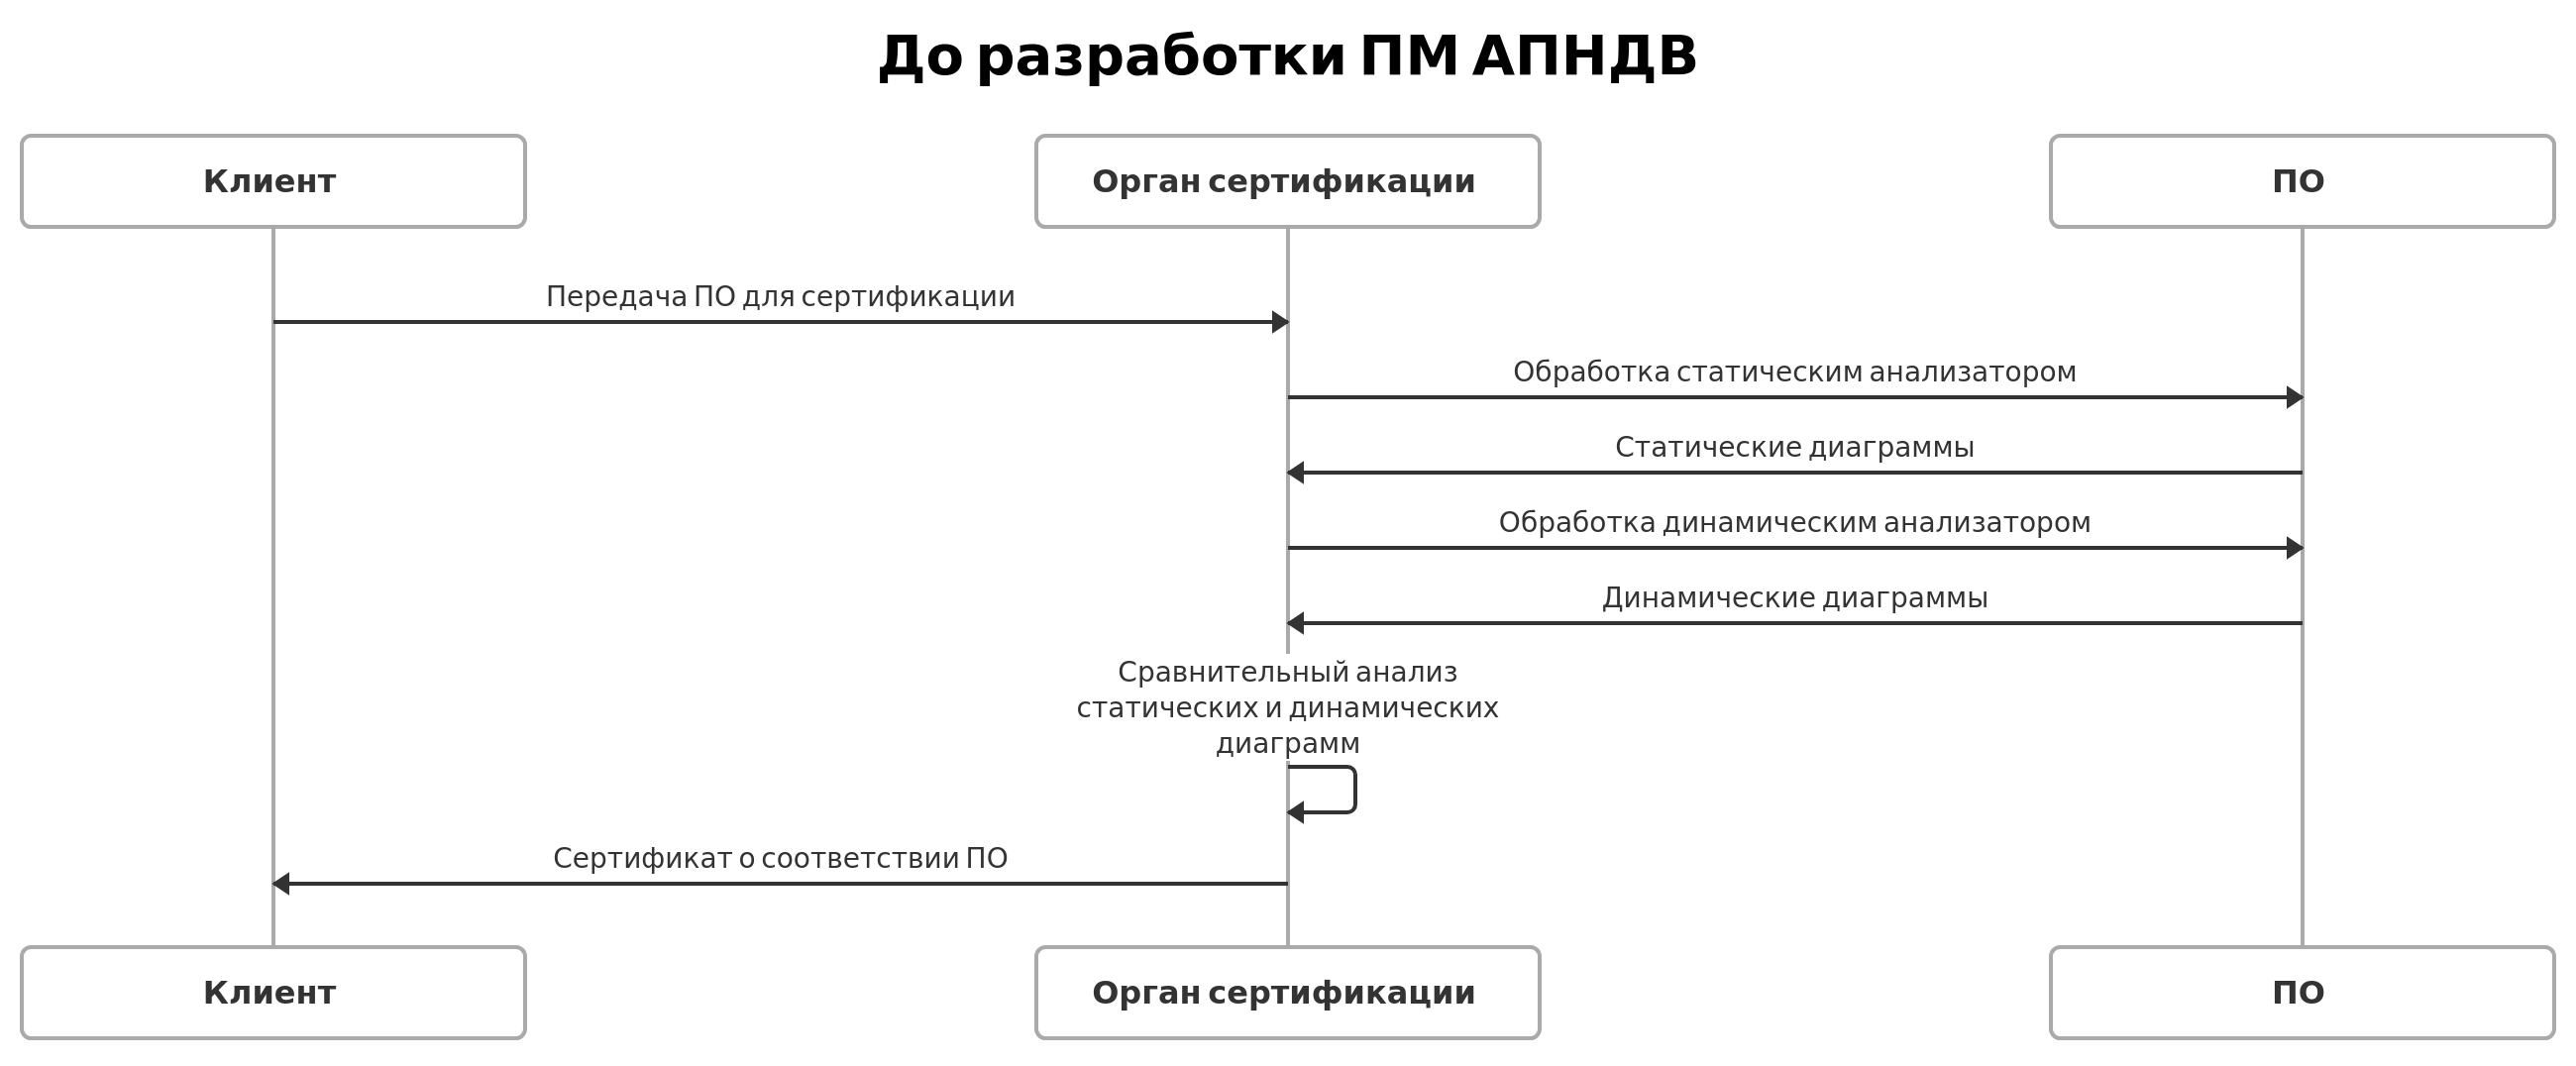
\includegraphics[width=\textwidth,height=\textheight,keepaspectratio]{images/uml_before_cropped.png}
    \end{figure}
    \begin{figure}[!htbp]
    \vspace{-2.6ex} 
        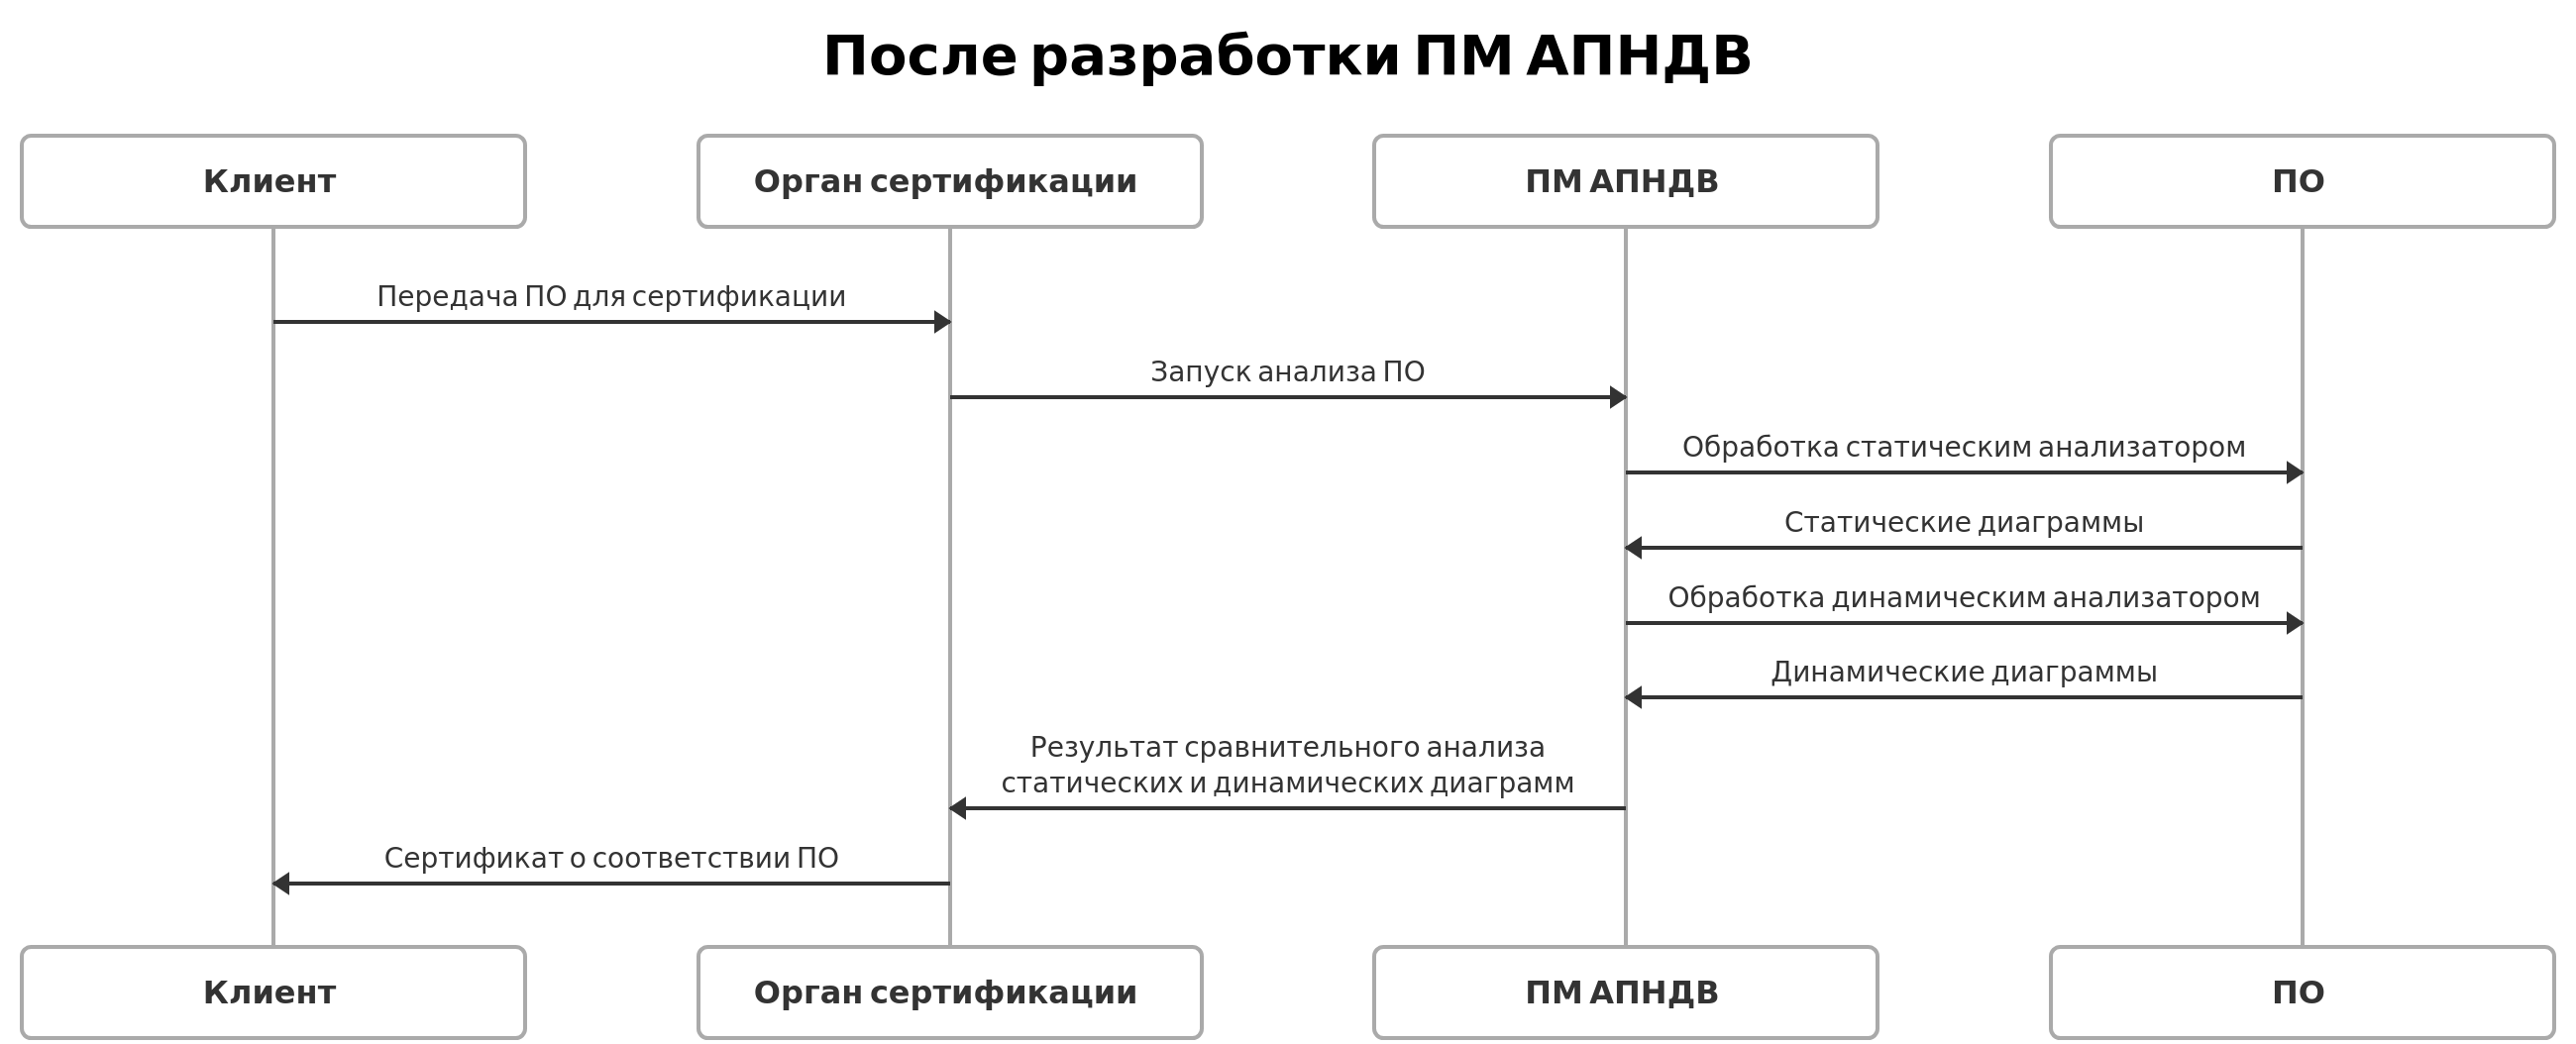
\includegraphics[width=\textwidth,height=\textheight,keepaspectratio]{images/uml_after_cropped.png}
    \end{figure}
%\begin{table}[!htbp]
%    \centering
%    \caption{\label{table:why-am-i-the-best}До и после разработки {\ProgModule}}
%
%    \begin{center}
%        \begin{tabular}{ | c | c | }
%            \hline
%            \makecell{До разработки {\ProgModule}} & \makecell{После разработки {\ProgModule}}\\
%            \hline
%            \makecell{Проведение статического,\\
%                      динамического и сравнительного\\
%                      анализа проходило вручную} & 
%            \makecell{Проведение статического,\\
%                      динамического и сравнительного\\
%                      анализа проходит автоматически}\\
%            \hline
%            \makecell{Для проведения анализов\\
%                      нужно было вручную выбирать\\
%                      исследуемые файлы} & 
%            \makecell{Для проведения анализов,\\
%                      {\ProgModule}\\
%                      делает это автоматически}\\
%            \hline
%            \makecell{Динамический анализ включал\\
%                      в себя только вызовы функций} & 
%            \makecell{Динамический анализ включает\\
%                      в себя информацию о состоянии\\
%                      стека и регистров программы\\
%                      во время конкретного вызова}\\
%            \hline
%        \end{tabular}
%    \end{center}
%
%\end{table}
\end{frame}

\begin{frame}%[plain, noframenumbering, t]
\frametitle{Обзор существующих решений}

Статические анализаторы.
\begin{table}[!htbp]
    {\footnotesize
        \setlength{\tabcolsep}{2pt}
        \begin{longtable}{*{4}{| c}|}
            \hline
            \diagbox[width=4cm]{Свойства}{Название\\программы}                                       &
            \makecell{Microsoft\\Application\\Inspector \autocite{microsoft-application-inspector}} &
            \makecell{SCI\\Tools\\Understand \autocite{sci-tools-understand}}                       &
            \makecell{GNU cflow \autocite{gnu-cflow}} \\
            \hline
            \makecell{Кросс-платформенность}             & \greencell{Да} & \greencell{Да} & \greencell{Да}\\
            \hline
            \makecell{Открытость\\исходного кода}        & \greencell{Да} & \redcell{Нет}   & \greencell{Да}\\
            \hline
            \makecell{Препроцессирование\\кода C/C++}    & \redcell{Нет}   & \greencell{Да} & \greencell{Да}\\
            \hline
            \makecell{Представление\\
                      препроцессорных директив как\\
                      вызов функций}                     & \redcell{Нет}   & \redcell{Нет}   & \greencell{Да}\\
            \hline
            \makecell{Создание графа вызовов}            & \redcell{Нет}   & \greencell{Да} & \greencell{Да} \\
            \hline
            \makecell{Создание обратного\\графа вызовов} & \redcell{Нет}   & \greencell{Да} & \greencell{Да}\\
            \hline
            \makecell{Бесплатность}                      & \greencell{Да} & \redcell{Нет}   & \greencell{Да}\\
            \hline
            \makecell{Графический интерфейс}             & Нет & Есть & Нет \\
            \hline
        \end{longtable}
    }
\end{table}

{\tiny
\begin{itemize}
    \item \fullcite{microsoft-application-inspector}
    \item \fullcite{sci-tools-understand}
    \item \fullcite{gnu-cflow}
\end{itemize}
}

\end{frame}

\begin{frame}%[plain, noframenumbering, t]
\frametitle{Обзор существующих решений}

Динамические анализаторы.
\begin{table}[!htbp]
    {\small
        \setlength{\tabcolsep}{2pt}
        \begin{longtable}{*{3}{| c}|}
            \hline
            \diagbox[width=8cm]{Свойства}{Название программы} &
            \makecell{GDB \autocite{gdb}}                     &
            \makecell{QEMU \autocite{qemu}}                   \\
            \hline
            \makecell{Кросс-платформенность}             & \greencell{Да} & \greencell{Да} \\
            \hline
            \makecell{Открытость исходного кода}        & \greencell{Да} & \greencell{Да} \\
            \hline
            \makecell{Возможность анализировать память} & \greencell{Да} & \greencell{Да} \\
            \hline
            \makecell{Возможность программно управлять} & \greencell{Да} & \greencell{Да} \\
            \hline
            \makecell{Возможность создавать 
                      собственные команды}               & \greencell{Да} & \redcell{Нет}   \\
            \hline
            \makecell{Возможность удаленной 
                      отладки}                           & \greencell{Да} & \redcell{Нет}   \\
            \hline
            \makecell{Бесплатность}                      & \greencell{Да} & \greencell{Да} \\
            \hline
            \makecell{Графический интерфейс}             & Есть & Есть \\
            \hline
        \end{longtable}
    }
\end{table}
{\tiny
\begin{itemize}
    \item \fullcite{gdb}
    \item \fullcite{qemu}
\end{itemize}
}
\end{frame}

\begin{frame}%[plain, noframenumbering, t]
\frametitle{Выбор языка программирования}

\begin{table}
    {\small
        \setlength{\tabcolsep}{2pt}
        \begin{longtable}{*{5}{| c}|}
            \hline
            \diagbox[width=5cm]{Свойства}{Язык} &
                \makecell{Nim \autocite{nim}} &
                \makecell{Python \autocite{python}} &
                \makecell{Perl \autocite{perl}} &
                \makecell{C/C++} \\
            \hline
                \makecell{Сверхвысокоуровневость} & 
                \greencell{Да} & 
                \greencell{Да} &
                \greencell{Да} &
                \redcell{Нет} \\
            \hline
                \makecell{Компилируется в\\машинный код} & 
                \greencell{Да} & 
                \redcell{Нет} &
                \redcell{Нет} &
                \greencell{Да} \\
            \hline
                \makecell{Количество функции в\\стандартной библиотеке} & 
                5585 & 
                638 &
                1338 &
                1224 \\
            \hline
                \makecell{Портируемость} & 
                \greencell{Есть} & 
                \greencell{Есть} &
                \greencell{Есть} &
                \yellowcell{\makecell{Есть,\\но неудобная}}\\
            \hline
                \makecell{Встроенная\\генерация документации} & 
                \greencell{Есть} & 
                \greencell{Есть} &
                \greencell{Есть} &
                \redcell{Нет}\\
            \hline
                \makecell{Статическая типизация} & 
                \greencell{Есть} & 
                \redcell{Нет} &
                \redcell{Нет} &
                \greencell{Есть}\\
            \hline
                \makecell{Автоматическое\\управление памятью} & 
                \greencell{Есть} & 
                \greencell{Есть} &
                \greencell{Есть} &
                \greencell{Есть} \\
            \hline
                \makecell{Обобщенное программирование} & 
                \greencell{Есть} & 
                \greencell{Есть} &
                \greencell{Есть} &
                \greencell{Есть} \\
            \hline
                \makecell{Метапрограммирование} & 
                \greencell{Есть} & 
                \greencell{Есть} &
                \greencell{Есть} &
                \greencell{Есть} \\
            \hline
                \makecell{Опыт использования} & 
                \greencell{Есть} & 
                \greencell{Есть} &
                \redcell{Нет} &
                \greencell{Есть} \\
            \hline
        \end{longtable}
    }
\end{table}
\vspace{-2ex}
{\tiny
\begin{itemize}
    \item \fullcite{nim}
    \item \fullcite{python}
    \item \fullcite{perl}
\end{itemize}
}
\end{frame}

\begin{frame}%[plain, noframenumbering, t]
\frametitle{Выбор среды разработки}

Для разработки на Nim существует несколько IDE и огромное количество
текстовых редакторов, часть которых рассмотрим ниже:

\begin{table}[!htbp]
    {\small
        \setlength{\tabcolsep}{2pt}
        \begin{longtable}{*{6}{| c}|}
            \hline
            \diagbox[width=4cm]{Свойства}{IDE/Редактор} &
                \makecell{Aporia \autocite{aporia-ide}} &
                \makecell{Atom \autocite{atom-ide}} &
                \makecell{Sublime\\Text \autocite{sublime-ide}} &
                \makecell{Visual\\Studio\\Code \autocite{vs-code-ide}} &
                \makecell{Vim \autocite{vim-ide}} \\
            \hline
                \makecell{Поддержка плагинов} & 
                \redcell{Нет} &
                \greencell{Да} & 
                \greencell{Да} &
                \greencell{Да} &
                \greencell{Да} \\
            \hline
                \makecell{Требователен к ресурсам} & 
                \greencell{Нет} & 
                \redcell{Да} & 
                \greencell{Нет} & 
                \redcell{Да} & 
                \greencell{Нет} \\ 
            \hline
                \makecell{Имеет продвинутую систему\\редактирования текста} & 
                \redcell{Нет} &
                \redcell{Нет} &
                \redcell{Нет} &
                \redcell{Нет} &
                \greencell{Да} \\
            \hline
                \makecell{Кросс-платформенность} & 
                \greencell{Есть} & 
                \greencell{Есть} &
                \greencell{Есть} &
                \greencell{Есть} &
                \greencell{Есть} \\
            \hline
                \makecell{Может работать\\без GUI} & 
                \redcell{Нет} &
                \redcell{Нет} &
                \redcell{Нет} &
                \redcell{Нет} &
                \greencell{Да} \\
            \hline
                \makecell{Восстановление после сбоев} & 
                \redcell{Нет} & 
                \greencell{Есть} &
                \greencell{Есть} &
                \greencell{Есть} &
                \greencell{Есть} \\
            \hline
                \makecell{Возможность выделять\\ключевые слова с помощью\\регулярных выражений} & 
                \redcell{Нет} & 
                \greencell{Есть} &
                \greencell{Есть} &
                \greencell{Есть} &
                \greencell{Есть} \\
            \hline
                \makecell{Опыт использования} & 
                \redcell{Нет} &
                \redcell{Нет} &
                \greencell{Есть} &
                \greencell{Есть} &
                \greencell{Есть} \\
            \hline
        \end{longtable}
    }
\end{table}

\vspace{-3ex}
{\tiny
\begin{itemize}
    \item \fullcite{aporia-ide}
    \item \fullcite{atom-ide}
    \item \fullcite{sublime-ide}
    \item \fullcite{vs-code-ide}
    \item \fullcite{vim-ide}
\end{itemize}
}
\end{frame}

\begin{frame}%[plain, noframenumbering, t]
\frametitle{Схема данных {\ProgModule}}
    \begin{figure}[!htbp]
            % !TEX encoding = UTF-8 Unicode
% Úτƒ-8 encoded
% http://www.linux.org.ru/forum/general/10357036
\tikzset{
    line/.style={draw, -latex'},
    every join/.style={line},
    u/.style={anchor=south},
    r/.style={anchor=west},
    fxd/.style={text width = 6em},
    it/.style={font={\small\itshape}},
    bf/.style={font={\small\bfseries}}

}
\tikzstyle{base} =
    [
        draw,
        on chain,
        on grid,
        align=center,
        minimum height=4ex,
        minimum width = 5ex,
        node distance = 6mm and 60mm,
        text badly centered,
        text width=5cm
    ]
\tikzstyle{coord} =
    [
        coordinate,
        on chain,
        on grid
    ]
\tikzstyle{cloud} =
    [
        base,
        ellipse,
        node distance = 3cm,
        minimum height = 2em
    ]
\tikzstyle{decision} =
    [
        base,
        diamond,
        aspect=2,
        node distance = 2cm,
        inner sep = 0pt
    ]
\tikzstyle{block} =
    [
        rectangle,
        base,
        rounded corners,
        minimum height = 2em
    ]
\tikzstyle{print_block} =
    [
        base,
        tape,
        tape bend top=none,
    ]
\tikzstyle{io} =
    [
        base,
        trapezium,
        trapezium left angle = 70,
        trapezium right angle = 110,
    ]
\tikzstyle{prompt} =
    [
        base,
        trapezium,
        trapezium left angle = 90,
        trapezium right angle = 80,
        shape border rotate = 90
    ]
\tikzstyle{disk file} =
    [
        base,
        cylinder,
        aspect=0.2,
    ]
\tikzstyle{process} =
    [
        rectangle,
        base,
    ]
\makeatletter
\pgfkeys{/pgf/.cd,
    subrtshape w/.initial=2mm,
    cycleshape w/.initial=2mm
}
\pgfdeclareshape{subrtshape}{
    \inheritsavedanchors[from=rectangle]
    \inheritanchorborder[from=rectangle]
    \inheritanchor[from=rectangle]{north}
    \inheritanchor[from=rectangle]{center}
    \inheritanchor[from=rectangle]{west}
    \inheritanchor[from=rectangle]{east}
    \inheritanchor[from=rectangle]{mid}
    \inheritanchor[from=rectangle]{base}
    \inheritanchor[from=rectangle]{south}
    \backgroundpath{
        \southwest \pgf@xa=\pgf@x \pgf@ya=\pgf@y
        \northeast \pgf@xb=\pgf@x \pgf@yb=\pgf@y
        \pgfmathsetlength\pgfutil@tempdima{\pgfkeysvalueof{/pgf/subrtshape w}}
        \def\ppd@offset{\pgfpoint{\pgfutil@tempdima}{0ex}}
        \def\ppd@offsetm{\pgfpoint{-\pgfutil@tempdima}{0ex}}
        \pgfpathmoveto{\pgfqpoint{\pgf@xa}{\pgf@ya}}
        \pgfpathlineto{\pgfqpoint{\pgf@xb}{\pgf@ya}}
        \pgfpathlineto{\pgfqpoint{\pgf@xb}{\pgf@yb}}
        \pgfpathlineto{\pgfqpoint{\pgf@xa}{\pgf@yb}}
        \pgfpathclose
        \pgfpathmoveto{\pgfpointadd{\pgfpoint{\pgf@xa}{\pgf@yb}}{\ppd@offsetm}}
        \pgfpathlineto{\pgfpointadd{\pgfpoint{\pgf@xa}{\pgf@ya}}{\ppd@offsetm}}
        \pgfpathlineto{\pgfpointadd{\pgfpoint{\pgf@xb}{\pgf@ya}}{\ppd@offset}}
        \pgfpathlineto{\pgfpointadd{\pgfpoint{\pgf@xb}{\pgf@yb}}{\ppd@offset}}
        \pgfpathclose
    }
}
\pgfdeclareshape{cyclebegshape}{
    \inheritsavedanchors[from=rectangle]
    \inheritanchorborder[from=rectangle]
    \inheritanchor[from=rectangle]{north}
    \inheritanchor[from=rectangle]{center}
    \inheritanchor[from=rectangle]{west}
    \inheritanchor[from=rectangle]{east}
    \inheritanchor[from=rectangle]{mid}
    \inheritanchor[from=rectangle]{base}
    \inheritanchor[from=rectangle]{south}
    \backgroundpath{
        \southwest \pgf@xa=\pgf@x \pgf@ya=\pgf@y
        \northeast \pgf@xb=\pgf@x \pgf@yb=\pgf@y
        \pgfmathsetlength\pgfutil@tempdima{\pgfkeysvalueof{/pgf/cycleshape w}}
        \pgfpathmoveto{\pgfqpoint{\pgf@xa}{\pgf@ya}}
\pgfpathlineto{\pgfpointadd{\pgfpoint{\pgf@xa}{\pgf@yb}}{\pgfpoint{0ex}{-\pgfutil@tempdima}}}
\pgfpathlineto{\pgfpointadd{\pgfpoint{\pgf@xa}{\pgf@yb}}{\pgfpoint{\pgfutil@tempdima}{0ex}}}
\pgfpathlineto{\pgfpointadd{\pgfpoint{\pgf@xb}{\pgf@yb}}{\pgfpoint{-\pgfutil@tempdima}{0ex}}}
\pgfpathlineto{\pgfpointadd{\pgfpoint{\pgf@xb}{\pgf@yb}}{\pgfpoint{0ex}{-\pgfutil@tempdima}}}
\pgfpathlineto{\pgfqpoint{\pgf@xb}{\pgf@ya}}
        \pgfpathclose
    }
}
\pgfdeclareshape{cycleendshape}{
    \inheritsavedanchors[from=rectangle]
    \inheritanchorborder[from=rectangle]
    \inheritanchor[from=rectangle]{north}
    \inheritanchor[from=rectangle]{center}
    \inheritanchor[from=rectangle]{west}
    \inheritanchor[from=rectangle]{east}
    \inheritanchor[from=rectangle]{mid}
    \inheritanchor[from=rectangle]{base}
    \inheritanchor[from=rectangle]{south}
    \backgroundpath{
        \southwest \pgf@xa=\pgf@x \pgf@ya=\pgf@y
        \northeast \pgf@xb=\pgf@x \pgf@yb=\pgf@y
        \pgfmathsetlength\pgfutil@tempdima{\pgfkeysvalueof{/pgf/cycleshape w}}
        \pgfpathmoveto{\pgfqpoint{\pgf@xb}{\pgf@yb}}
\pgfpathlineto{\pgfpointadd{\pgfpoint{\pgf@xb}{\pgf@ya}}{\pgfpoint{0ex}{\pgfutil@tempdima}}}
\pgfpathlineto{\pgfpointadd{\pgfpoint{\pgf@xb}{\pgf@ya}}{\pgfpoint{-\pgfutil@tempdima}{0ex}}}
\pgfpathlineto{\pgfpointadd{\pgfpoint{\pgf@xa}{\pgf@ya}}{\pgfpoint{\pgfutil@tempdima}{0ex}}}
\pgfpathlineto{\pgfpointadd{\pgfpoint{\pgf@xa}{\pgf@ya}}{\pgfpoint{0ex}{\pgfutil@tempdima}}}
\pgfpathlineto{\pgfqpoint{\pgf@xa}{\pgf@yb}}
        \pgfpathclose
    }
}
\makeatother
\tikzstyle{subroutine} =
    [
        base,
        subrtshape,
    ]
\tikzstyle{cyclebegin} =
    [
        base,
        cyclebegshape,
    ]
\tikzstyle{cycleend} =
    [
        base,
        cycleendshape,
    ]
\tikzstyle{connector} =
    [
        base,
        circle,
    ]
\begin{tikzpicture}[%
    start chain=going below,    % General flow is top-to-bottom
    node distance=6mm and 30mm, % Global setup of box spacing
    scale=0.7, 
    every node/.style={scale=0.72}
    ] 
        \node [prompt   ] (makefile path)   [left  = 2cm ]                               {\small Путь до папки с Makefile};
        \node [process  ] (builder)         [below = 0.7cm of makefile path]             {\small Сборщик};
        \node [disk file] (makefile)        [yshift=0.5cm, left  = 5cm of makefile path] {\small Makefile};
        \node [prompt   ] (executable)      [right = 10cm of makefile path]              {\small Путь до исполняемого файла};
        \node [process  ] (breakpointer)                                                 {\small Модуль бинарного анализа};
        \node [disk file] (modified exe)    [xshift=3.5cm, below = 1cm of breakpointer]  {\small Модифицированный исполняемый файл};
        \node [disk file] (build log)       [xshift=3.5cm, below = 1cm of builder]       {\small Файл с информацией о сборке};
        \node [disk file] (call map)        [left = 8.25cm of build log]                 {\small Файл с информацией о линковке};
        \node [process  ] (static analyzer) [below = 1.25cm of build log]                {\small Модуль статического анализа};
        \node [disk file] (sources)         [left = 4.15cm of build log]                 {\small Файлы с исходным кодом};
        \node [disk file] (gdb script)      [left = 5cm of modified exe]                 {\small Скрипт для GDB};
        \node [process  ] (gdb manager)     [below = 2.25cm of breakpointer]             {\small Модуль управления отладчиком};
        \node [disk file] (dyn result)      [below = 1.25cm of gdb manager]              {\small Результаты динамического анализа};
        \node [process  ] (dyn parser)      [below = 1.25cm of dyn result]               {\small Модуль преобразования результатов динамического анализа};
        \node [disk file] (dyn json)        [below = 1.25cm of dyn parser]               {\small Преобразованные результаты динамического анализа};
        \node [disk file] (stat result)     [below = 1.25cm of static analyzer]          {\small Результаты статического анализа};
        \node [process  ] (stat parser)     [below = 1.25cm of stat result]              {\small Модуль преобразования результатов статического анализа};
        \node [disk file] (stat json)       [below = 1.25cm of stat parser]              {\small Преобразованные результаты статического анализа};
        \node [process  ] (aggregator)      [below = 1.25cm of stat json]                {\small Модуль агрегирования результатов линковки и статического анализа};
        \node [disk file] (aggregator file) [below = 1.25cm of aggregator]               {\small Агрегированные результаты линковки и статического анализа};
        \node [process  ] (comparer)                                                     {\small Модуль сравнительного анализа};
        \node [disk file] (summary)                                                      {\small Результаты сравнительного анализа};
        \node [disk file] (file executable) [left = 4.5cm of executable]                 {\small Исполняемый\\файл};

        \draw [-] (makefile path)      -- (builder);
        \draw [-] (makefile)           -- +(0,-0.95) -| (builder);
        \draw [line] (builder)         -| (call map);
        \draw [line] (builder)         -| (build log);

        \draw [line] (executable)      -- (breakpointer);
        \draw [line] (file executable) -- +(0,-0.7) -| (breakpointer);
        \draw [line] (breakpointer)    -| (modified exe);
        \draw [line] (breakpointer)    -| (gdb script);

        \draw [line] (modified exe)    |- (gdb manager);
        \draw [line] (gdb script)      |- (gdb manager);
        \draw [line] (gdb manager)     -- (dyn result);
        \draw [line] (dyn result)      -- (dyn parser);
        \draw [line] (dyn parser)      -- (dyn json);


        \draw [line] (build log)       -- (static analyzer);
        \draw [line] (static analyzer) -- (stat result);
        \draw [line] (stat result)     -- (stat parser);
        \draw [line] (stat parser)     -- (stat json);
        \draw [line] (call map)        |- (aggregator);
        \draw [line] (stat json)       -- (aggregator);
        \draw [line] (aggregator)      -- (aggregator file);
        \draw [line] (sources)         |- (static analyzer);

        \draw [line] (aggregator file) -- (comparer);
        \draw [line] (dyn json)        |- (comparer);
        \draw [line] (comparer)        -- (summary);

\end{tikzpicture}

    \end{figure}
\end{frame}

\begin{frame}%[plain, noframenumbering, t]
\frametitle{Схема алгоритма {\ProgModule}}

    \Put(149,-490){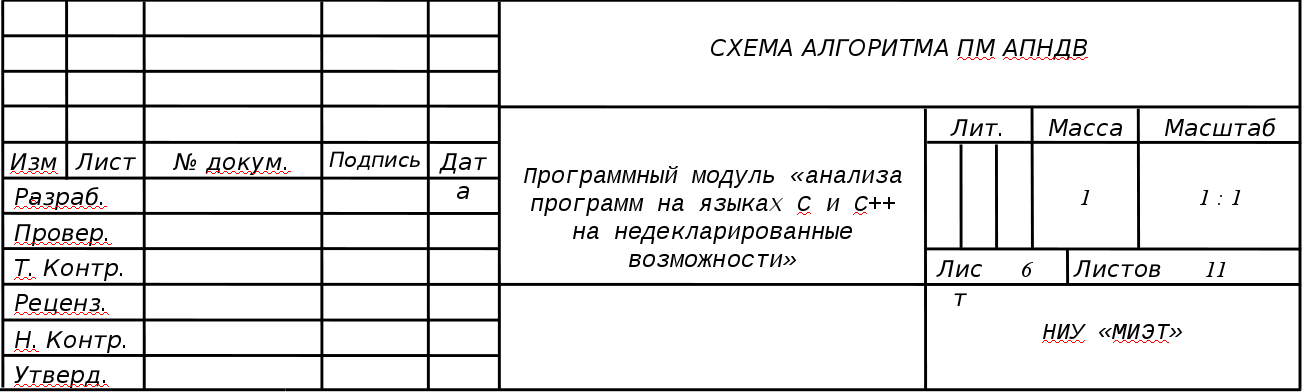
\includegraphics[height=2cm]{Presentation/images/algo_gost.png}}
    %\begin{figure}[!htbp]
    %    \begin{adjustbox}{max totalsize={1.0\textwidth}{0.8\textheight},left}
    %        \includegraphics{}
    %    \end{adjustbox}
    %\end{figure}

    \begin{figure}[!htbp]
        \vspace{-1ex} 
        \hspace{-13cm} 
        \begin{adjustbox}{max totalsize={1.6\textwidth}{1.6\textheight},left}
            % !TEX encoding = UTF-8 Unicode
% Úτƒ-8 encoded
% http://www.linux.org.ru/forum/general/10357036
\tikzset{
    line/.style={draw, -latex'},
    every join/.style={line},
    u/.style={anchor=south},
    r/.style={anchor=west},
    fxd/.style={text width = 6em},
    it/.style={font={\small\itshape}},
    bf/.style={font={\small\bfseries}},
}
\tikzstyle{base_long} =
    [
        draw,
        on chain,
        on grid,
        align=center,
        minimum height=4ex,
        minimum width = 10ex,
        node distance = 6mm and 60mm,
        text badly centered,
    ]
\tikzstyle{base} =
    [
        draw,
        on chain,
        on grid,
        align=center,
        minimum height=4ex,
        minimum width = 10ex,
        node distance = 6mm and 60mm,
        text badly centered,
        text width=5cm
    ]
\tikzstyle{coord} =
    [
        coordinate,
        on chain,
        on grid
    ]
\tikzstyle{cloud} =
    [
        base,
        ellipse,
        node distance = 3cm,
        minimum height = 2em,
        text width=2cm
    ]
\tikzstyle{decision} =
    [
        base,
        diamond,
        aspect=2,
        node distance = 2cm,
        inner sep = 0pt
    ]
\tikzstyle{block} =
    [
        rectangle,
        base,
        rounded corners,
        minimum height = 2em
    ]
\tikzstyle{print_block} =
    [
        base,
        tape,
        tape bend top=none,
    ]
\tikzstyle{io} =
    [
        base,
        trapezium,
        trapezium left angle = 70,
        trapezium right angle = 110,
    ]
\tikzstyle{prompt} =
    [
        base,
        trapezium,
        trapezium left angle = 90,
        trapezium right angle = 80,
        shape border rotate = 90
    ]
\tikzstyle{disk file} =
    [
        base,
        cylinder,
        aspect=0.2,
    ]
\tikzstyle{process} =
    [
        rectangle,
        base,
    ]
\makeatletter
\pgfkeys{/pgf/.cd,
    subrtshape w/.initial=2mm,
    cycleshape w/.initial=2mm
}
\pgfdeclareshape{parallelshape}{
    \inheritsavedanchors[from=rectangle]
    \inheritanchorborder[from=rectangle]
    \inheritanchor[from=rectangle]{north}
    \inheritanchor[from=rectangle]{center}
    \inheritanchor[from=rectangle]{west}
    \inheritanchor[from=rectangle]{east}
    \inheritanchor[from=rectangle]{mid}
    \inheritanchor[from=rectangle]{base}
    \inheritanchor[from=rectangle]{south}
    \backgroundpath{
        \southwest \pgf@xa=\pgf@x \pgf@ya=\pgf@y
        \northeast \pgf@xb=\pgf@x \pgf@yb=\pgf@y
        \def\ppd@offset{\pgfpoint{\pgfutil@tempdima}{0ex}}
        \def\ppd@offsetm{\pgfpoint{-\pgfutil@tempdima}{0ex}}
        \pgfpathmoveto{\pgfqpoint{\pgf@xa}{\pgf@ya}}
            \pgfpathlineto{\pgfqpoint{\pgf@xb}{\pgf@ya}}
        \pgfpathclose
        \pgfpathmoveto{\pgfqpoint{\pgf@xb}{\pgf@yb}}
            \pgfpathlineto{\pgfqpoint{\pgf@xa}{\pgf@yb}}
        \pgfpathclose
    }
}
\pgfdeclareshape{subrtshape}{
    \inheritsavedanchors[from=rectangle]
    \inheritanchorborder[from=rectangle]
    \inheritanchor[from=rectangle]{north}
    \inheritanchor[from=rectangle]{center}
    \inheritanchor[from=rectangle]{west}
    \inheritanchor[from=rectangle]{east}
    \inheritanchor[from=rectangle]{mid}
    \inheritanchor[from=rectangle]{base}
    \inheritanchor[from=rectangle]{south}
    \backgroundpath{
        \southwest \pgf@xa=\pgf@x \pgf@ya=\pgf@y
        \northeast \pgf@xb=\pgf@x \pgf@yb=\pgf@y
        \pgfmathsetlength\pgfutil@tempdima{\pgfkeysvalueof{/pgf/subrtshape w}}
        \def\ppd@offset{\pgfpoint{\pgfutil@tempdima}{0ex}}
        \def\ppd@offsetm{\pgfpoint{-\pgfutil@tempdima}{0ex}}
        \pgfpathmoveto{\pgfqpoint{\pgf@xa}{\pgf@ya}}
        \pgfpathlineto{\pgfqpoint{\pgf@xb}{\pgf@ya}}
        \pgfpathlineto{\pgfqpoint{\pgf@xb}{\pgf@yb}}
        \pgfpathlineto{\pgfqpoint{\pgf@xa}{\pgf@yb}}
        \pgfpathclose
        \pgfpathmoveto{\pgfpointadd{\pgfpoint{\pgf@xa}{\pgf@yb}}{\ppd@offsetm}}
        \pgfpathlineto{\pgfpointadd{\pgfpoint{\pgf@xa}{\pgf@ya}}{\ppd@offsetm}}
        \pgfpathlineto{\pgfpointadd{\pgfpoint{\pgf@xb}{\pgf@ya}}{\ppd@offset}}
        \pgfpathlineto{\pgfpointadd{\pgfpoint{\pgf@xb}{\pgf@yb}}{\ppd@offset}}
        \pgfpathclose
    }
}
\pgfdeclareshape{cyclebegshape}{
    \inheritsavedanchors[from=rectangle]
    \inheritanchorborder[from=rectangle]
    \inheritanchor[from=rectangle]{north}
    \inheritanchor[from=rectangle]{center}
    \inheritanchor[from=rectangle]{west}
    \inheritanchor[from=rectangle]{east}
    \inheritanchor[from=rectangle]{mid}
    \inheritanchor[from=rectangle]{base}
    \inheritanchor[from=rectangle]{south}
    \backgroundpath{
        \southwest \pgf@xa=\pgf@x \pgf@ya=\pgf@y
        \northeast \pgf@xb=\pgf@x \pgf@yb=\pgf@y
        \pgfmathsetlength\pgfutil@tempdima{\pgfkeysvalueof{/pgf/cycleshape w}}
        \pgfpathmoveto{\pgfqpoint{\pgf@xa}{\pgf@ya}}
\pgfpathlineto{\pgfpointadd{\pgfpoint{\pgf@xa}{\pgf@yb}}{\pgfpoint{0ex}{-\pgfutil@tempdima}}}
\pgfpathlineto{\pgfpointadd{\pgfpoint{\pgf@xa}{\pgf@yb}}{\pgfpoint{\pgfutil@tempdima}{0ex}}}
\pgfpathlineto{\pgfpointadd{\pgfpoint{\pgf@xb}{\pgf@yb}}{\pgfpoint{-\pgfutil@tempdima}{0ex}}}
\pgfpathlineto{\pgfpointadd{\pgfpoint{\pgf@xb}{\pgf@yb}}{\pgfpoint{0ex}{-\pgfutil@tempdima}}}
\pgfpathlineto{\pgfqpoint{\pgf@xb}{\pgf@ya}}
        \pgfpathclose
    }
}
\pgfdeclareshape{cycleendshape}{
    \inheritsavedanchors[from=rectangle]
    \inheritanchorborder[from=rectangle]
    \inheritanchor[from=rectangle]{north}
    \inheritanchor[from=rectangle]{center}
    \inheritanchor[from=rectangle]{west}
    \inheritanchor[from=rectangle]{east}
    \inheritanchor[from=rectangle]{mid}
    \inheritanchor[from=rectangle]{base}
    \inheritanchor[from=rectangle]{south}
    \backgroundpath{
        \southwest \pgf@xa=\pgf@x \pgf@ya=\pgf@y
        \northeast \pgf@xb=\pgf@x \pgf@yb=\pgf@y
        \pgfmathsetlength\pgfutil@tempdima{\pgfkeysvalueof{/pgf/cycleshape w}}
        \pgfpathmoveto{\pgfqpoint{\pgf@xb}{\pgf@yb}}
\pgfpathlineto{\pgfpointadd{\pgfpoint{\pgf@xb}{\pgf@ya}}{\pgfpoint{0ex}{\pgfutil@tempdima}}}
\pgfpathlineto{\pgfpointadd{\pgfpoint{\pgf@xb}{\pgf@ya}}{\pgfpoint{-\pgfutil@tempdima}{0ex}}}
\pgfpathlineto{\pgfpointadd{\pgfpoint{\pgf@xa}{\pgf@ya}}{\pgfpoint{\pgfutil@tempdima}{0ex}}}
\pgfpathlineto{\pgfpointadd{\pgfpoint{\pgf@xa}{\pgf@ya}}{\pgfpoint{0ex}{\pgfutil@tempdima}}}
\pgfpathlineto{\pgfqpoint{\pgf@xa}{\pgf@yb}}
        \pgfpathclose
    }
}
\makeatother
\tikzstyle{subroutine} =
    [
        base,
        subrtshape,
    ]
\tikzstyle{cyclebegin} =
    [
        base,
        cyclebegshape,
    ]
\tikzstyle{cycleend} =
    [
        base,
        cycleendshape,
    ]
\tikzstyle{connector} =
    [
        base,
        circle,
    ]

\tikzstyle{parallel} =
    [
        base_long,
        parallelshape,
    ]
\begin{tikzpicture}[%
    start chain=going below,    % General flow is top-to-bottom
    node distance=6mm and 30mm, % Global setup of box spacing
    ] 
        \node [cloud    ] (makefile)        [left  = 4cm ]                   {\small Начало};
        \node [process  ] (builder)         [below = 1cm of makefile]        {\small Сборщик};
        \node [parallel ] (parallel)        [below of = builder, yscale=0.3] {\rptf[105]{\ }};
        \node [process  ] (breakpointer)    [below right = 5cm of builder]   {\small Бинарный анализ};
        \node [process  ] (static analyzer) [below left = 5cm of builder]    {\small Статический анализ};
        \node [process  ] (stat parser)     [below = 2cm of static analyzer] {\small Преобразование результатов статического анализа};
        \node [process  ] (aggregator)      [below = 2cm of stat parser]     {\small Агрегирование результатов линковки и статического анализа};
        \node [process  ] (gdb manager)     [below = 2cm of breakpointer]    {\small Динамический анализ};
        \node [process  ] (dyn parser)      [below = 2cm of gdb manager]     {\small Преобразование результатов динамического анализа};
        \node [cloud    ] (end)             [below = 15cm of makefile]       {\small Конец};
        \node [process  ] (comparer)        [above = 2cm of end]             {\small Сравнительный анализ};
        \node [parallel ] (parallel aggr)   [above = 2cm of comparer, yscale=0.3] {\rpts[105]{\ }};

        \draw [line] (makefile) -- (builder);
        \draw [-] (builder)     -- (parallel);

        \draw [-] (parallel)  -- +(-3.55,-0.095) -- +(-3.55,-1.2) -- (static analyzer);
        \draw [-] (parallel)  -- +(+3.55,-0.095) -- +(+3.55,-1.2) -- (breakpointer);

        \draw [line] (static analyzer) -- (stat parser);
        \draw [line] (stat parser)     -- (aggregator);

        \draw [line] (breakpointer)    -- (gdb manager);
        \draw [line] (gdb manager)     -- (dyn parser);

        \draw [-] (aggregator) -- +(+0,-1.05) -- +(+0,-2.37) -- (parallel aggr);
        \draw [-] (dyn parser) -- +(-0,-1.09) -- +(-0,-2.37) -- (parallel aggr);
        \draw [-] (parallel aggr) -- (comparer);
        \draw [line] (comparer)   -- (end);

\end{tikzpicture}

        \end{adjustbox}
        %\caption{Схема алгоритма {\ProgModule}\label{fig:algorithm}}
    \end{figure}
\end{frame}

\begin{frame}%[plain, noframenumbering, t]
\frametitle{Пользовательский интерфейс {\ProgModule}}
    Пользователь может управлять {\ProgModule}, как с помощью
    консольного интерфейса, так и графического.
    \begin{figure}[!htbp]
        \begin{adjustbox}{max totalsize={0.8\textwidth}{0.8\textheight}}
            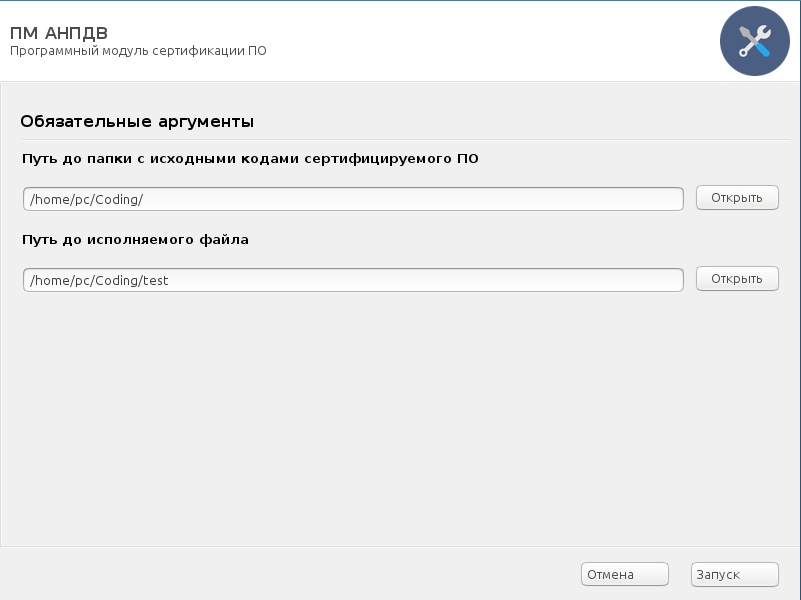
\includegraphics[trim={0.2em 0.2ex 0.2ex 0.2ex},clip,width=\linewidth]{images/apndv-gui.png}
        \end{adjustbox}
        %\caption{Схема алгоритма {\ProgModule}\label{fig:algorithm}}
    \end{figure}

\end{frame}

\begin{frame}%[plain, noframenumbering, t]
\frametitle{Отладка и тестирование {\ProgModule}}
    В процессе разработки {\ProgModule} было написано 32 модульных теста, рассматривающих
    различные сценарии использования элементов {\ProgModule}. {\ProgModule} отлаживался
    с помощью отладчика GDB.
    
    \vspace{3ex}
    \begin{figure}[!htbp]
        \begin{adjustbox}{max totalsize={1.2\textwidth}{1.2\textheight}}
            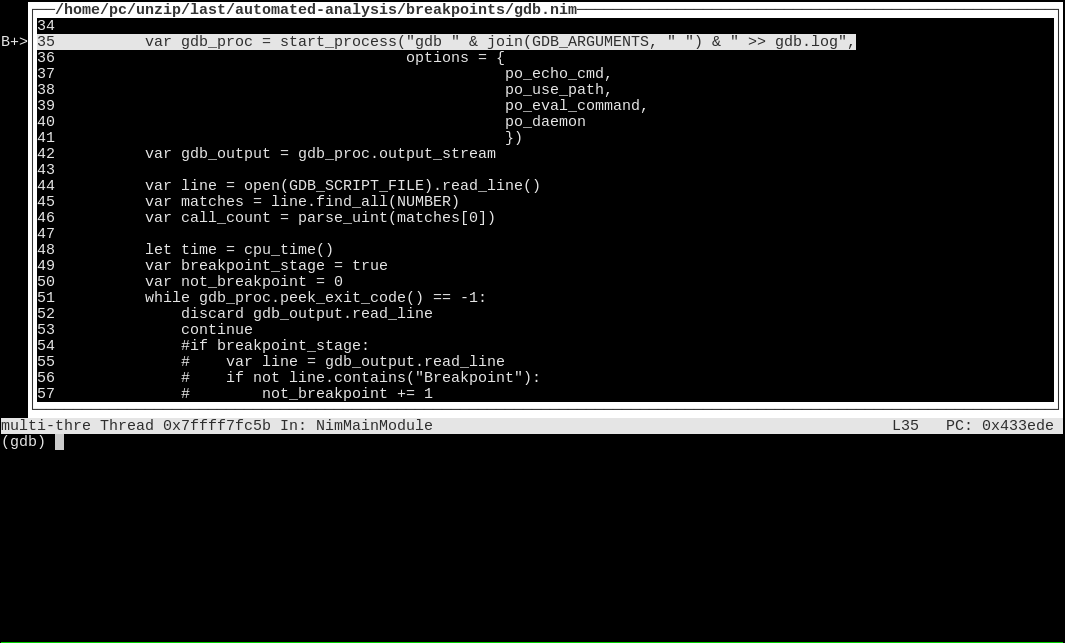
\includegraphics[trim={0 4ex 0 0 0},clip,width=\linewidth]{images/running-gdb.png}
        \end{adjustbox}
        %\caption{Схема алгоритма {\ProgModule}\label{fig:algorithm}}
    \end{figure}

\end{frame}

\begin{frame}%[plain, noframenumbering, t]
\frametitle{Апробация}
    \begin{itemize}
        \item Уманский А.А. Разработка coreutils на языке Forth для встраиваемых систем.
            <<Актуальные проблемы информатизации в цифровой жкономике и научных исследованиях>>
            Международная научно-практическая конференция 2019
    \end{itemize}
\end{frame}

\begin{frame}%[plain, noframenumbering, t]
\frametitle{Результаты работы}
    \begin{itemize}
        \item исследована предметная область;
        \item проведен сравнительный анализ существующих программных решений;
        \item выборан язык и среда разработки;
        \item разработана схема данных {\ProgModule};
        \item разработана схема алгоритма {\ProgModule};
        \item запрограммирован {\ProgModule};
        \item проведена отладка и тестирование {\ProgModule};
        \item разработано руководство оператора к {\ProgModule};
    \end{itemize}
    Цель ВКР достигнута.
\end{frame}

\begin{frame}%[plain, noframenumbering, t]

    \begin{center}
        \Huge Спасибо за внимание!
    \end{center}
    
\end{frame}
